{\chapter{Physical Design of Graph Data Structures}
\label{chap:PhysicalDesign}

In (\ref{chap:Background}),  we  presented  the  necessary  background  knowledge  concerning  topics covered in this thesis.  In this chapter, we dive deep into the main topic of this thesis by presenting the set of evaluation questions we are going to answer in this thesis as well as the physical design of the graph data structures, we are going to evaluate. This chapter is consisted of the following sections:
\begin{itemize}  
\item \textbf{Evaluation Questions:}\\
First, we introduce a set of evaluation questions, we intend to answer in this thesis in (\ref{sec:EvalQuests}).

\item\textbf{Graph Topology Structures:}\\
In (\ref{sec:PhyDesign-GraphTopology}), we present the physical design of a set of data structures that can be used by graph databases for the storage of a graph topology.

\item\textbf{Graph Properties Structures:}\\
We present the physical design of a set of data structures that can be used by graph databases for the storage of a graph properties in (\ref{sec:PhyDesign-GraphProperties}).

\item\textbf{Concurrent Graph Structures:}\\
In (\ref{sec:PhyDesign-ConcurrentGraphStructs}), we present the physical design of a concurrent version of the adjacency list and the Nested Key-Value Store graph data structures.

\item\textbf{Graph Partitioning:}\\
Next, we present a method for partitioning the graph topology in order to support an edge-labeled multi-graph in (\ref{sec:PhyDesign-GraphPartitioning}).

\item \textbf{Summary:}\\
Finally, we provide a summary the main topics we discussed in this chapter in (\ref{sec:PhyDesign-Summary}).
\end{itemize}



\section{Evaluation Questions}
\label{sec:EvalQuests}

A set of data structures has been developed over time for the purpose of efficient storage and processing of graph data. Although, all the graph data structures can perform the same tasks, their performance is highly dependent on the characteristics of the data as well as the kind of computation performed on this data \cite{Paradies2017}.

In a survey performed by (\textit{Sahu et al.}), the authors have mentioned a list of challenges for processing a graph. On top of the list of challenges came scalability. The scalability of loading, updating and performing computations on a large graph is the most prevalent issue challenge for graph processing systems \cite{sahu2017ubiquity}.

In this thesis we are going to answer a set of evaluation questions that focuses on the effect of the use of a specific data structure for storing graph data on the performance. Following are the concrete set of evaluation questions we aim to answer in this thesis:

\begin{enumerate}
%Pardon the mess in the notes.
\item How do the execution time for loading data, and the memory footprint, scale for the different graph data structures when they need to accommodate larger data sizes (i.e. higher number of vertices and/or edges)? 
%We agreed that the results reducing files are Ok for SF1. But we also want changes in SFs, such that we really can compare scales. We hope 0.1, 0.5... And being evil, I would even suggest 5 and 10. 
%Suggestion for writing Q1 differently: How do the execution time for loading data, and the memory footprint, scale for the different data structures when they need to accommodate larger data sizes (i.e. higher number of vertices and/or edges)? 
\item What is the impact of loading the data in large versus small batches, for the different graph data structures, on the performance on this task?
\item What change in the data loading time, could processing the data in parallel introduce in comparison to sequential processing?
%We will test only with one data structure. And we agree on this. But we need to make a good argument why we choose this data structure, and also why just one. 
%Data sizes perhaps (but here we can prune and maybe only have 3 sizes)
\item Given a selection and centrality queries, what is the effect of the the data structure choice on the query response time?%matching queries
%We could test with different sizes too.
%Selection query: centrality.
%Then your 4th chapter will be: Memory Footprint Scalability and Data Loading
%Then your 5th chapter will be: Data Structure Suitability 
%for Matching and Selection Queries
%Future work: Mining queries... And interactive workloads.

%Pointer to help you elaborate the questions for queries: http://citeseerx.ist.psu.edu/viewdoc/download?doi=10.1.1.721.9607&rep=rep1&type=pdf
\end{enumerate}

For answering the above set of questions, we implemented the graph data structures previously introduced in (\ref{sec:StorageStructures}). We have used \textit{C++} as the programming language for our implementation. We utilized the standard \textit{C++} data structures library (\textit{Standard Template Library (STL)}) for building up the graph data structures (for more information on \textit{C++} or $STL$, see \cite{josuttis2012c++}). 

In (\ref{sec:PhyDesign-GraphTopology}, \ref{sec:PhyDesign-GraphProperties}, \ref{sec:PhyDesign-ConcurrentGraphStructs}, and \ref{sec:PhyDesign-GraphPartitioning}), we present the detailed physical design for the different implemented graph data structures. We have implemented all the data structures for in-memory processing of data with no involvement of disk persistent storage. 

In (\ref{chap:Eval_4} and \ref{chap:Eval_5}), we present the evaluation results of tests we have executed on our implemented graph data structures. Also, we present answers for the above mentioned evaluation questions based on the findings from the evaluation tests.


\begin{figure}[H]
\centering
    \subfigure[Vertex-labeled directed graph $G$.]
    {
        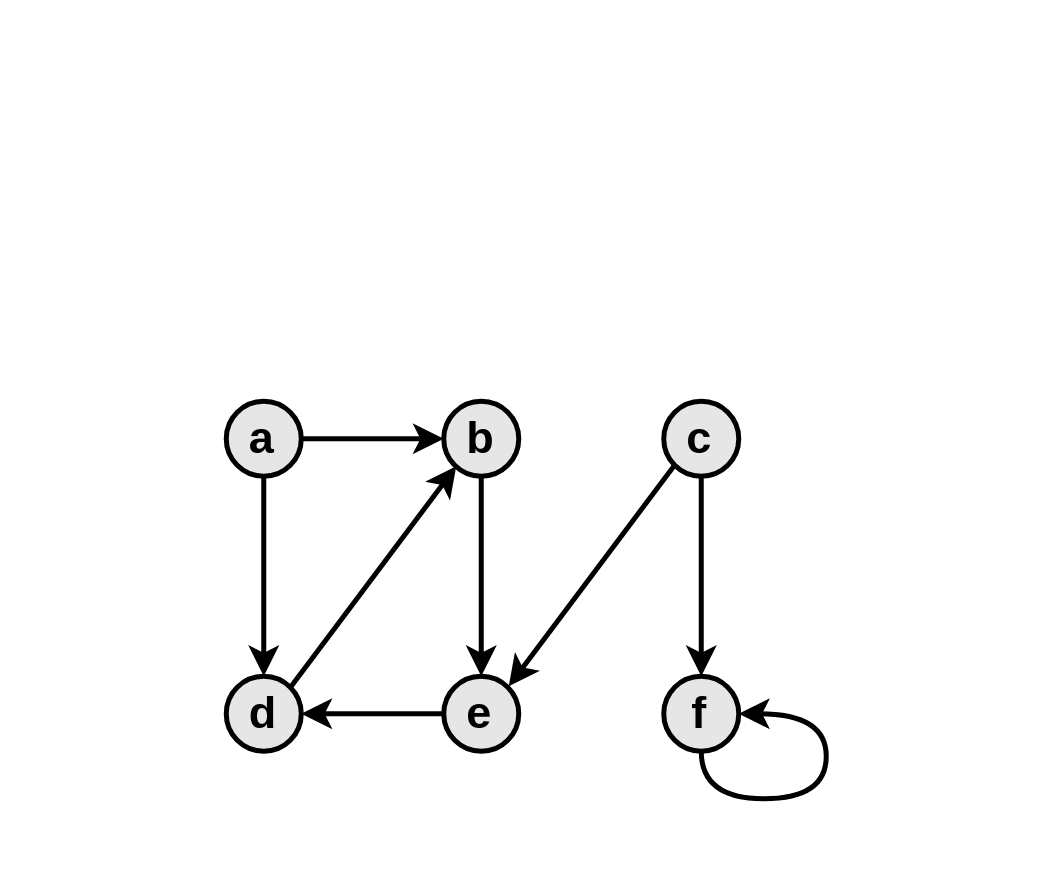
\includegraphics[width=0.4\textwidth]{pics/DirectedGraph_Alpha.png}
        \label{fig:DirectedGraph_Alpha}
    }
\centering
    \subfigure[Auxiliary vertex-label look-up index.]
    {
        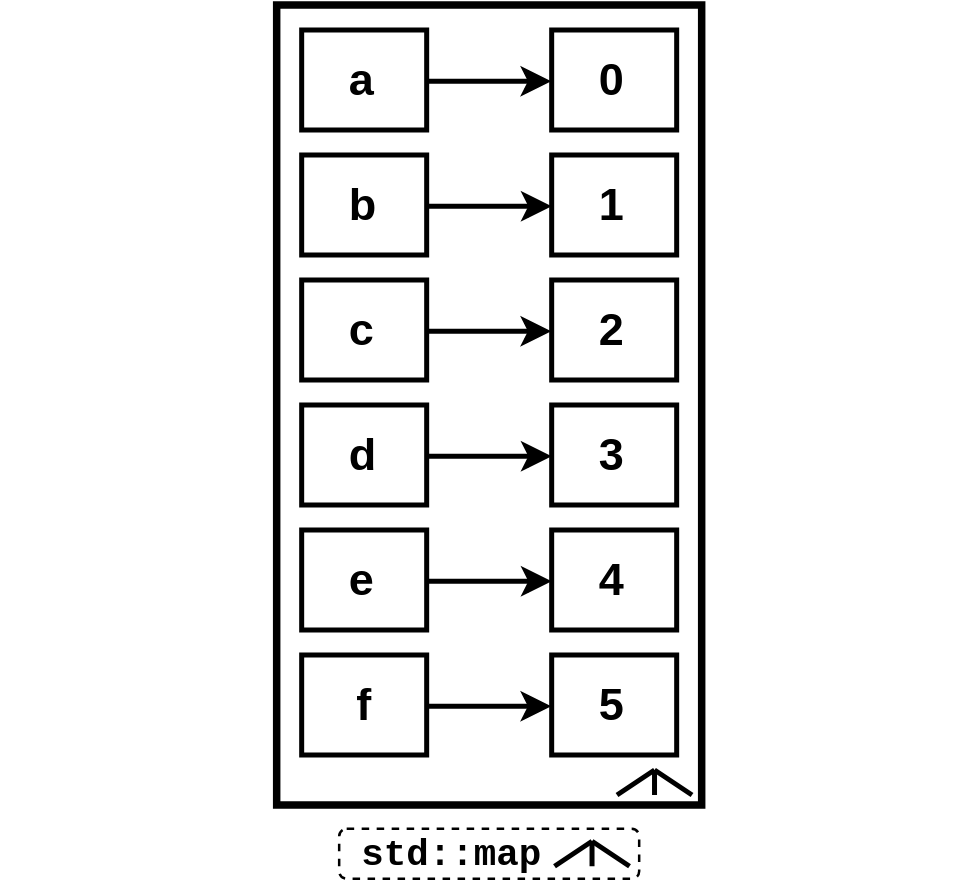
\includegraphics[width=0.4\textwidth]{pics/AdjacencyMatrix_Aux_Physical.png}
        \label{fig:AdjMat_Aux_phy}
    }
\centering
    \subfigure[Adjacency matrix physical representation of $G$.]
    {
        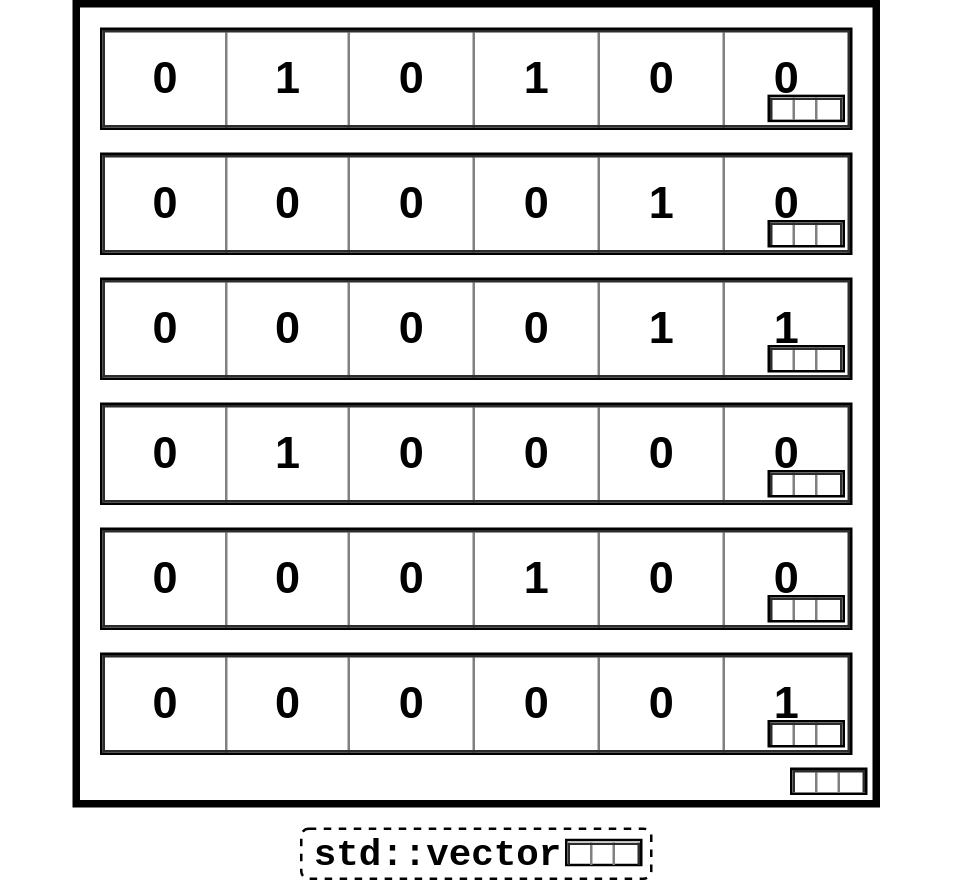
\includegraphics[width=0.42\textwidth]{pics/AdjacencyMatrix_Physical.png}
        \label{fig:AdjMat_phy}
    }
\centering
    \subfigure[CSR physical representation of $G$.]
    {
        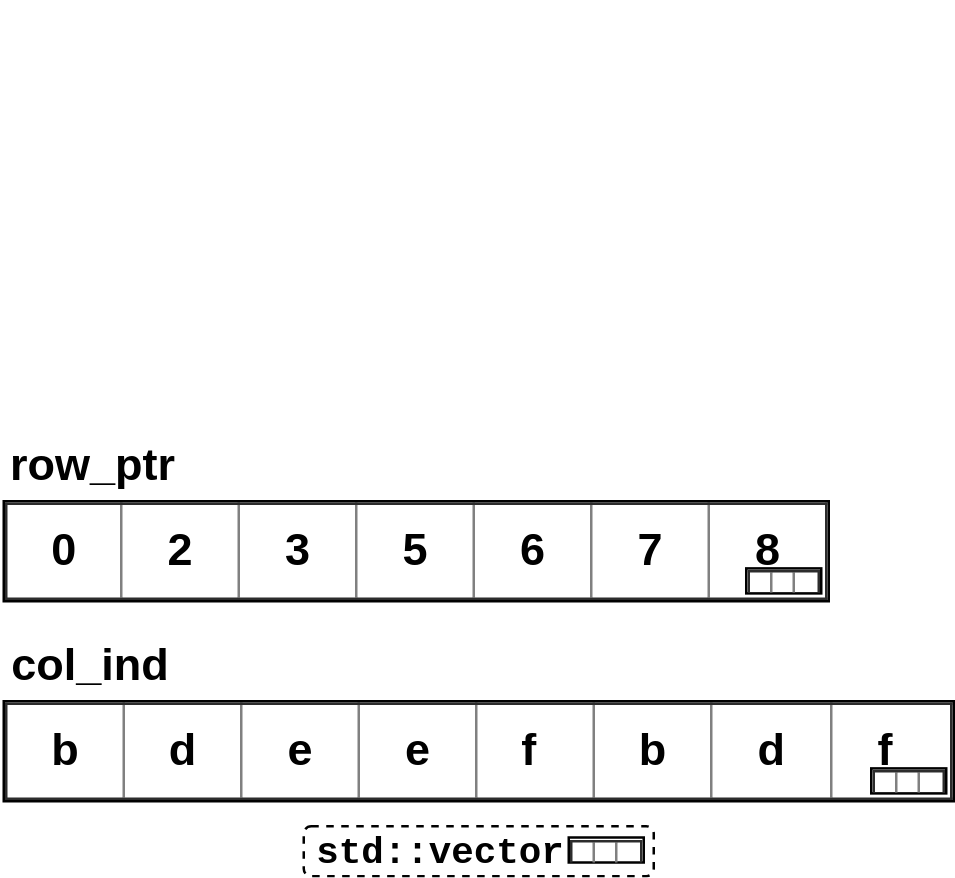
\includegraphics[width=0.4\textwidth]{pics/CSR_Physical.png}
        \label{fig:CSR_phy}
    }
\centering
    \subfigure[Adjacency list physical representation of $G$.]
    {
        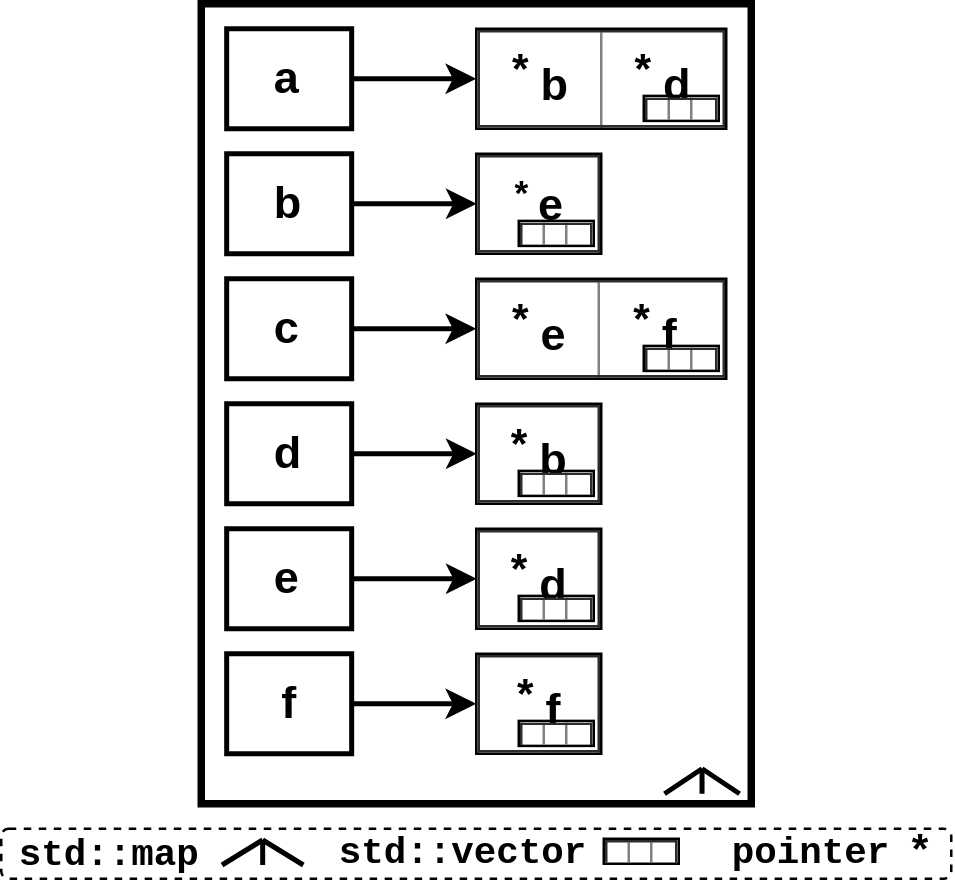
\includegraphics[width=0.4\textwidth]{pics/AdjacencyList_Physical.png}
        \label{fig:AdjLst_phy}
    }
    \caption{Physical representations of the topology of vertex-labeled directed graph \textit{G}.}
    \label{fig:GraphRopology_physical}
\end{figure}


\section{Graph Topology Structures}
\label{sec:PhyDesign-GraphTopology}

In (\ref{sec:EvalQuests}), we introduced a set of evaluation questions that we aim to answer in this thesis. In this section, we present the physical design of graph topology data structures we implemented , which we later will execute a set of evaluation tests on to find an answer for the evaluation questions.

We have used the \textit{C++} programming language in the implementation of the data structures. We have utilized data structures from the $C++-STL$ library as the base for designing and implementing the graph topology data structures. We have implemented all the data structures for in-memory processing of data with no involvement of disk persistent storage (for more information on \textit{C++} or $STL$, see \cite{josuttis2012c++}).

Following, we present the physical design of the three graph topology data structures (adjacency matrix, compressed sparse row (CSR), and adjacency list) in (\ref{subsec:PhyDesign-AdjacencyMatrix}, \ref{subsec:PhyDesign-CSR}, and \ref{subsec:PhyDesign-AdjacencyList}) respectively.



\subsection{Adjacency Matrix}
\label{subsec:PhyDesign-AdjacencyMatrix}

In (\ref{subsubsec:AdjacencyMatrix}), we have presented the necessary background knowledge on adjacency matrices. We have discussed the logical design, suitable usage scenarios, and the memory requirements of the adjacency matrix data structure. We will present in this section our physical design of adjacency matrix.

We designed the adjacency matrix physically in a way that maintains its logical definition. We constructed adjacency matrix using the (\texttt{std::vector}) data structure in $C++$. Elements in (\texttt{std::vector}) are placed in sequence and are accessed using their index. The (\texttt{std::vector}) allocates its elements in consecutive memory locations which offers better data locality. Also, (\texttt{std::vector})'s are able to dynamically re-size to store new data. Those three characteristics have made (\texttt{std::vector}) the best choice for the design of adjacency matrix \cite{josuttis2012c++}.

We represent each row in the adjacency matrix using a single (\texttt{std::vector}), with all of the (\texttt{std::vector})'s that represent the rows, have the same size equal to the number of vertices forming the graph. We grouped all the (\texttt{std::vector})'s that are representing the adjacency matrix rows into another (\texttt{std::vector}).

In a vertex-labeled directed graph, each vertex is labeled with a unique label. The vertex label doesn't has to be a numeric label, however the label can be constructed using a string of characters. The adjacency matrix logical design however, is assuming a numeric labeled vertices. To solve this problem, we attached an auxiliary structure to the adjacency matrix. The purpose of the auxiliary structure is to serve as a look-up index by mapping each unique vertex-label to a unique number that represents the vertex's both row-and-column index in the adjacency matrix.
\\
\\

In (Figure \ref{fig:AdjMat_phy}, we show an example of the adjacency matrix physical representation of the vertex-labeled directed graph $G$ shown in (Figure \ref{fig:DirectedGraph_Alpha}). The 6x6 adjacency matrix in the figure is constructed using a set of (\texttt{std::vector})'s grouped into another (\texttt{std::vector}). In (Figure \ref{fig:AdjMat_Aux_phy}), we show we show the auxiliary vertex-label look-up index that maps each vertex-label in $G$ to a unique number representing the vertex's both row-and-column index in the adjacency matrix.



\subsection{Compressed Sparse Row (CSR)}
\label{subsec:PhyDesign-CSR}

In (\ref{subsubsec:CSR}), we have presented the necessary background knowledge on the compressed sparse row (CSR) structure. We have discussed the logical design, suitable usage scenarios, and the memory requirements of CSR. We will present in this section our physical design of the compressed sparse row (CSR).

For constructing the compressed sparse row (CSR) we needed a data structure that is able to place elements in a sequence with access to the elements using their position, store the elements in consecutive memory locations for better data locality, and offers a dynamic size feature for accommodating new data. The (\texttt{std::vector}) data structure is matching the needed requirements and hence we choose it for the physical design of CSR \cite{josuttis2012c++}.

The compressed sparse row (CSR) physical design is consisted of two (\texttt{std::vector})'s. The first (\texttt{std::vector}) is representing the \textit{row\_ptr} structure and the second (\texttt{std::vector}) is representing the \textit{col\_ind} structure.

CSR inherits the same issue that adjacency matrix faces with a vertex-labeled directed graph, where each vertex is not limited to numeric labels but also can be labeled using a string of characters. We solve this issue in the same way we solved it in adjacency matrix by attaching an auxiliary structure to the CSR. The purpose of the auxiliary structure is to serve as a look-up index by mapping each unique vertex-label to a unique number that represents the original vertex's both row-and-column index in the adjacency matrix. As the vertex-label and the column index in the adjacency matrix are no-longer equal, we chosen to directly store the vertex-label rather than the column index in the \textit{col\_ind} structure.

In (Figure \ref{fig:CSR_phy}, we show an example of the compressed sparse row (CSR) physical representation of the vertex-labeled directed graph $G$ shown in (Figure \ref{fig:DirectedGraph_Alpha}). The CSR physical structure in the figure is constructed using one (\texttt{std::vector}) representing the \textit{row\_ptr} structure and another (\texttt{std::vector}) representing the \textit{col\_ind} structure. In (Figure \ref{fig:AdjMat_Aux_phy}), we show we show the auxiliary vertex-label look-up index that maps each vertex-label in $G$ to a unique number representing the original vertex's both row-and-column index in the adjacency matrix.


\subsection{Adjacency List}
\label{subsec:PhyDesign-AdjacencyList}





\section{Graph Properties Structures}
\label{sec:PhyDesign-GraphProperties}




\subsection{Universal Table}
\label{subsec:PhyDesign-UniversalTable}


\subsection{Emerging Schema}
\label{subsec:PhyDesign-EmergingSchema}


\subsection{Nested Key-Value Store}
\label{subsec:PhyDesign-NestedStore}



\section{Concurrent Graph Structures}
\label{sec:PhyDesign-ConcurrentGraphStructs}


\subsection{Concurrent Adjacency List}
\label{subsec:PhyDesign-ConcurrentAdjacencyList}


\subsection{Concurrent Nested Key-Value Store}
\label{subsec:PhyDesign-ConcurrentNestedStore}



\section{Graph Partitioning}
\label{sec:PhyDesign-GraphPartitioning}



\section{Summary}
\label{sec:PhyDesign-Summary}




}